% !LW recipe = latexmk (latexmkrc)
%% Colloquium on the Machine -- the full deck (one PDF).
%% Build:  latexmk colloquium_on_the_machine.tex
%%   (lualatex, two passes; see .latexmkrc). Never latexmk -pdf.
%% Theme: sharedAssets/beamer/beamerthemetuftedark.sty. Layout catalogue in
%% sharedAssets/beamer/demo.tex, which layout for which content in
%% slidedesign.md, theme API in AGENTS.md.
%%
%% FORMAT. Two meetings per round. Meeting one: the three candidate books
%% (one novel, one educational, one different angle), the group picks one.
%% Three months of reading. Meeting two: 135 minutes of discussion along the
%% guiding questions of the chosen book. The Shelf then records the round:
%% the book read, the collective Likert verdict, the best quotes.
%%
%% ROUND 1 candidates: Hyperion (Simmons), How the Mind Works (Pinker),
%% The Beautiful Risk of Education (Biesta).
%%
%% Covers: NOT the publishers' covers, which are copyrighted. Each book gets
%% one public-domain image, pre-cropped to the 0.33 side strip (aspect
%% 0.587) as images/cover_<name>.jpg, all from Wikimedia Commons:
%%   cover_hyperion  File:Hyperion PIA07740.jpg, Saturn's moon Hyperion,
%%                   Cassini 2005, NASA/JPL, public domain
%%   cover_pinker    File:PurkinjeCell.jpg, Ramon y Cajal, Purkinje cells
%%                   of the pigeon cerebellum, 1899, public domain (d. 1934)
%%   cover_biesta    File:Georges de La Tour - The Magdalen with the Smoking
%%                   Flame - Google Art Project-cropped.jpg, c. 1640, LACMA,
%%                   public domain
%% Until a file exists, \bookcover draws a placeholder box and \bookside
%% the gray placeholder strip with the file name as caption.
\documentclass[aspectratio=169]{beamer}
\usetheme{tuftedark}
% The Intelligence Engineering layout: footer with name and progress track,
% \sidecaption up the strip edge, flush-left takeaway, \framesubtitle.
\input{tuftedarklayout}
\usepackage{pgfplotstable}% the Likert verdict reads its counts from a table

% Drop slide images in images/; include by bare name, e.g.
%   \includegraphics[width=\linewidth]{machine}
\graphicspath{{images/}}

% Placeholder image: \phimg[width-fraction]{label}. Draws a labeled box in place
% of an image not yet made; swap for \includegraphics once the asset exists.
\newcommand{\phimg}[2][0.5]{%
  \tikz\node[draw=tddim, thick, rounded corners, fill=tddim!12,
    minimum width={#1*\linewidth}, minimum height={0.62*#1*\linewidth},
    inner sep=4pt, align=center, text=tddim,
    font=\ttfamily\scriptsize]{\detokenize{#2}};%
}

% Book covers. \ifcover{name}{found}{missing} tests images/name.jpg|png.
\newcommand{\ifcover}[3]{%
  \IfFileExists{images/#1.jpg}{#2}{\IfFileExists{images/#1.png}{#2}{#3}}}
% \bookcover[lift]{name}: the image as a square tile for the overview row,
% every tile the same size: the strip image at tile width, cropped to the
% square. [lift] moves the image up by that fraction of the tile, to choose
% which part of a tall image shows (0 = its middle). A placeholder box of
% the same size carries the file name until the image exists.
\newlength{\coverht}
\setlength{\coverht}{0.21\textheight}
\newcommand{\bookcover}[2][0]{%
  \ifcover{#2}{%
    \begin{tikzpicture}
      \clip (0,0) rectangle (\coverht,\coverht);
      \node[inner sep=0pt] at (0.5\coverht,{(0.5+#1)*\coverht})
        {\includegraphics[width=\coverht]{#2}};
    \end{tikzpicture}}{%
    \tikz\node[draw=tddim, thick, rounded corners, fill=tddim!12,
      minimum width={\coverht}, minimum height={\coverht},
      inner sep=2pt, align=center, text=tddim,
      font=\ttfamily\scriptsize]{\detokenize{#2}};}}
% \bookside{name}{credit}: the image as the full-height 0.33 side strip of a
% book's detail frame, its credit (source and licence) as the \sidecaption;
% the gray placeholder strip with the file name until the image exists.
\newcommand{\bookside}[2]{%
  \ifcover{#1}{\sideimagecover[0.33]{#1}\sidecaption{#2}}{%
    \sideimagecover[0.33]{placeholder_gray.png}%
    \sidecaption{\detokenize{#1}}}}

% One line of book facts as the frame subtitle, under the title.
\newcommand{\bookfacts}[1]{\framesubtitle{#1}}
% Sets a sidebody ragged right and unhyphenated, so the narrow column never
% breaks a word. Call it first in the sidebody.
\newcommand{\pitchtext}{\raggedright\hyphenpenalty=10000 }
% The question a book puts to us, in red. Unused since the detail frames
% became plain pitches; their red is one \alert phrase in the description.
\newcommand{\bookquestion}[1]{\par\bigskip{\usebeamercolor[fg]{alerted text}#1}}

% The book the round read. Set it once the vote is in; the Shelf frames pick
% it up.
\newcommand{\chosenbook}{chosen book}

% \quotenote{quote}: one quote as a margin-note block, in the theme's own
% margin style (tdmargin: dim grey, margin size), set in a 0.30 column so
% three sit side by side. No names. The starred form \quotenote*{quote}
% sets the one red quote of the frame, the best of the six.
\NewDocumentCommand{\quotenote}{sm}{%
  \begin{tdmargin}%
    \IfBooleanT{#1}{\usebeamercolor[fg]{alerted text}}%
    ``#2''%
  \end{tdmargin}}

\title[Colloquium on the Machine]{Colloquium on the Machine}
\author[Schutera]{Prof.\ Dr.-Ing.\ Mark Schutera}
\institute{\textcolor{DHBWred}{DHBW}\ Ravensburg}
\date{\today}
\setbookversion{\today}{upbeat plantain Habicht}

% Section dividers from the second section on: the title page leads straight
% into the choice of book, the later sections open on a divider.
\AtBeginSection[]{%
  \ifnum\value{section}>1
    \begin{frame}\sectionpage\end{frame}%
  \fi}

\begin{document}

% The title frame of colloquium_on_the_machine.tex, which inputs this file.
% The title page is the course poster on white: the poster's statue
% (figures/poster/make_title_statue.py) beside the theme's title block, whose
% last line is broken in two so it ends left of the statue. The braces keep
% the white page and the dark text on this one frame.
{%
\setbeamercolor{title}{fg=black}
\setbeamercolor{author}{fg=DHBWgray}
\setbeamercolor{institute}{fg=DHBWgray}
\usebackgroundtemplate{%
  \begin{tikzpicture}
    \useasboundingbox (0,0) rectangle (\paperwidth,\paperheight);
    \fill[white] (0,0) rectangle (\paperwidth,\paperheight);
    \node[anchor=south east,inner sep=0pt] at (\paperwidth,3mm)
      {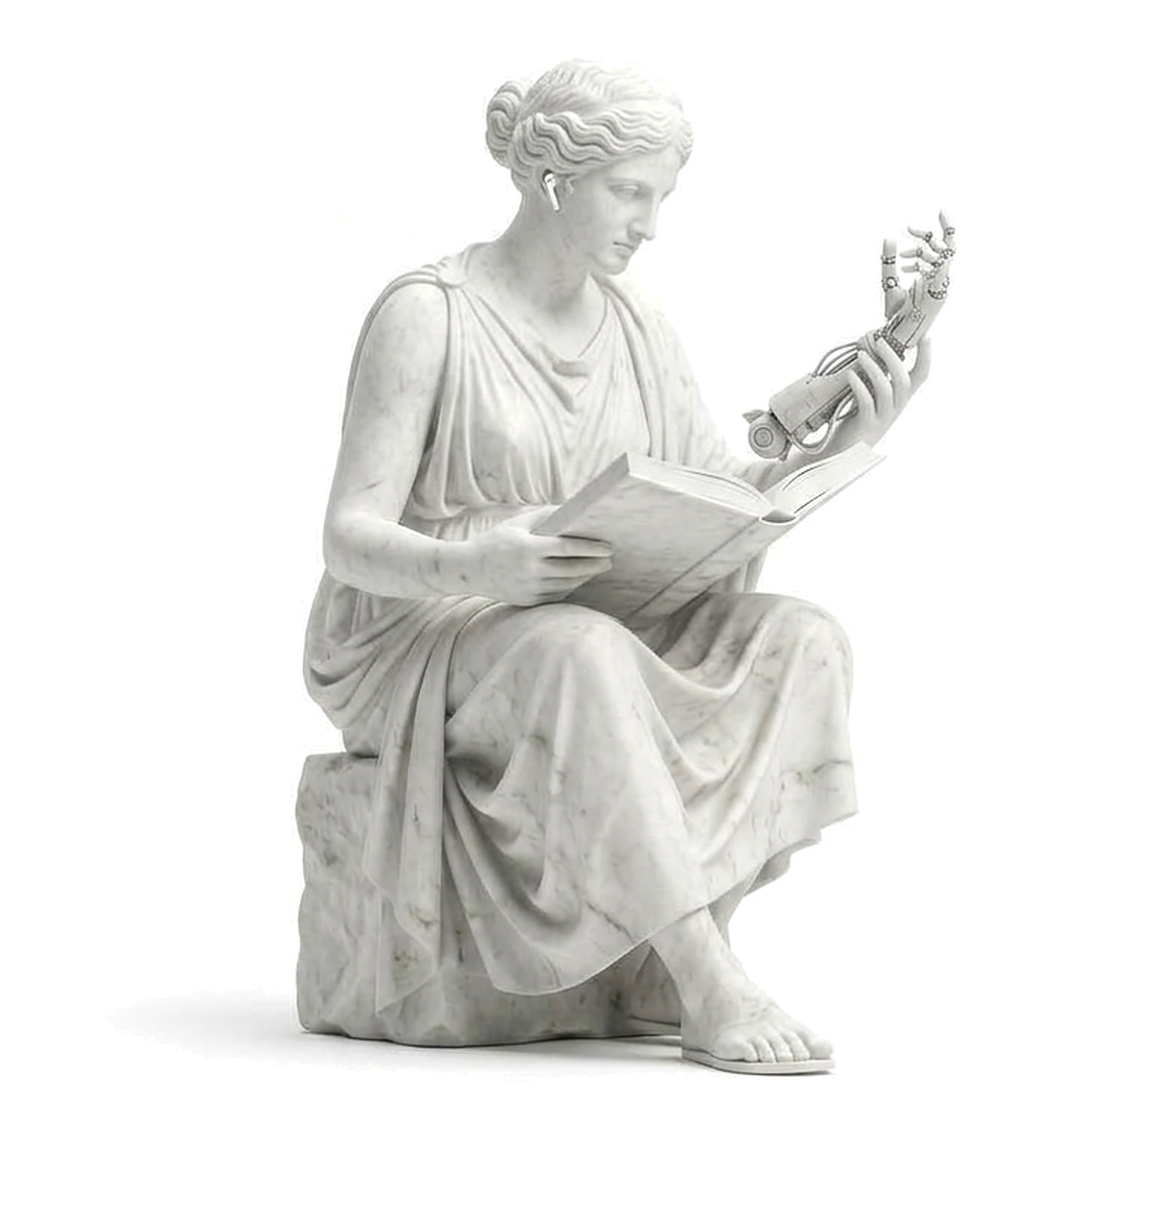
\includegraphics[height=0.95\paperheight]{title_statue}};
    \node[anchor=south east,inner sep=0pt,font=\tiny,text=DHBWgray]
      at (\paperwidth-3mm,3mm) {Image created with Google Gemini};
  \end{tikzpicture}}
\setbeamertemplate{title page}{%
  \vskip2mm%
  {\small\usebeamercolor[fg]{institute}\insertinstitute}\par%
  \vfill
  {\color{DHBWred}\rule{0.16\paperwidth}{2pt}}\par\vskip0.8em%
  {\usebeamerfont{title}\usebeamercolor[fg]{title}\inserttitle\par}%
  \vskip3em%
  {\normalsize\usebeamercolor[fg]{author}\insertauthor\par
    \vskip0.3em\printbookversion\par}%
  \vfill
}
\begin{frame}[plain]
  \titlepage
\end{frame}}
% the poster's statue on white

% ======================================================================
\section{Three Books}
% ======================================================================

% How the session runs, explained once up front. The same five steps return
% on the last frame of the section, there with the three books.
\begin{frame}{How We Choose}
  \centering
  \begin{tikzpicture}[td, node distance=7mm,
      gloss/.style={text=tddim, font=\scriptsize, align=center,
        text width=23mm, inner sep=0pt}]
    \node[tdbox] (pitch) {Pitch};
    \node[tdbox, right=of pitch] (research) {Research};
    \node[tdbox, right=of research] (commit) {Commit};
    \node[tdbox, right=of commit] (discuss) {Discuss};
    \node[tdboxhi, right=of discuss] (vote) {Vote};
    \draw[tdarr] (pitch) -- (research);
    \draw[tdarr] (research) -- (commit);
    \draw[tdarr] (commit) -- (discuss);
    \draw[tdarr] (discuss) -- (vote);
    \node[gloss, below=3mm of pitch] {three books};
    \node[gloss, below=3mm of research] {look into them yourself};
    \node[gloss, below=3mm of commit] {make up your mind};
    \node[gloss, below=3mm of discuss] {argue for your book};
    \node[gloss, below=3mm of vote] {everyones opinion counts};
  \end{tikzpicture}
  \par\bigskip\bigskip
  “When you read, don’t just consider what the author thinks,
  consider what you think.”\end{frame}

\begin{frame}{Hyperion}
  \bookfacts{Dan Simmons \textperiodcentered{} 1989 \textperiodcentered{}
      novel \textperiodcentered{} 482 pages, about 37 a week}
  \bookside{cover_hyperion}{Hyperion, NASA/JPL, public domain}
  \begin{sidebody}
    \pitchtext
    % Own pitch (Mark's pick, 2026-11-20), on the AI side of the novel.
    Humanity lives on hundreds of worlds linked by portals it did not
    build itself. The \alertbf{AIs} run them, advise the
    government, and keep their own plans to themselves. When tech advances to mix with religious fundamentalism, belief systems and doubts.
  \end{sidebody}
\end{frame}

\begin{frame}{How the Mind Works}
  \bookfacts{Steven Pinker \textperiodcentered{} 1997 \textperiodcentered{}
      science \textperiodcentered{} 660 pages, about 51 a week}
  \bookside{cover_pinker}{Ram\'on y Cajal, 1899, public domain}
  \begin{sidebody}
    \pitchtext
    % Pinker's own statement of the book's key idea, verbatim.
    The mind is a system of \alertbf{organs of computation}, designed by
    natural selection to solve the kinds of problems our ancestors faced
    in their foraging way of life. The human mind from an organic compute substrate.
  \end{sidebody}
\end{frame}

\begin{frame}{The Beautiful Risk of Education}
  \bookfacts{Gert Biesta \textperiodcentered{} 2013 \textperiodcentered{}
      philosophy \textperiodcentered{} 178 pages, about 14 a week}
  \bookside{cover_biesta}{G.\ de La Tour, c.\ 1640, public domain}
  \begin{sidebody}
    \pitchtext
    % Goodreads description, second sentence verbatim.
    The risk is there because, as W. B. Yeats has put it, education is not
    about filling a bucket but about \alertbf{lighting a fire}. Sometimes it's worth looking at ones own role 
    from a different angle. So what is a student? How is education done right? 
  \end{sidebody}
\end{frame}

% The overview comes LAST: the group has heard all three pitches and sees the
% three books side by side. Then four steps, all on this frame:
%   research  everyone looks into the three books on their own
%   commit    each student commits to one book, anonymously, on a slip
%   discuss   open discussion with the overview on screen
%   vote      anonymous ranked paper ballot: 1st = 2 points, 2nd = 1,
%             3rd = 0, highest total wins, a tie goes to the book with
%             more first places. The vote decides; the commit
%             shows how the discussion moved the room.
% Slips for commit and vote: ballots.tex.


\begin{frame}{How We Choose}
  \centering
  \begin{tikzpicture}[td, node distance=7mm,
      gloss/.style={text=tddim, font=\scriptsize, align=center,
        text width=23mm, inner sep=0pt}]
    \node[tdbox] (pitch) {\_};
    \node[tdbox, right=of pitch] (research) {Research};
    \node[tdbox, right=of research] (commit) {Commit};
    \node[tdbox, right=of commit] (discuss) {Discuss};
    \node[tdboxhi, right=of discuss] (vote) {Vote};
    \draw[tdarr] (pitch) -- (research);
    \draw[tdarr] (research) -- (commit);
    \draw[tdarr] (commit) -- (discuss);
    \draw[tdarr] (discuss) -- (vote);
    \node[gloss, below=3mm of pitch] {\_\_};
    \node[gloss, below=3mm of research] {look into them yourself};
    \node[gloss, below=3mm of commit] {make up your mind};
    \node[gloss, below=3mm of discuss] {argue for your book};
    \node[gloss, below=3mm of vote] {everyones opinion counts};
  \end{tikzpicture}
  \par\bigskip\bigskip
  “When you read, don’t just consider what the author thinks,
  consider what you think.”\end{frame}



\newcommand{\tdstep}{{\color{tddim}$\rightarrow$}}
\begin{frame}{Let's Vote}
  
  \par\smallskip
  Rank all three on your slip, no name: First place 2 points, second 1,
  third 0. Most points wins, a tie goes to the book with more second places. If you cast a vote you are commited to read the book and prepare for the discussion at the end of the semester.
  
  \par\medskip
  \begin{columns}[T,onlytextwidth]
    \begin{column}{0.31\textwidth}\centering
      \bookcover{cover_hyperion}\par\smallskip
      {\color{tddim}Novel}\par
      \textbf{Hyperion}\par
      Dan Simmons
    \end{column}
    \begin{column}{0.31\textwidth}\centering
      \bookcover{cover_pinker}\par\smallskip
      {\color{tddim}Science}\par
      \textbf{How the Mind Works}\par
      Steven Pinker
    \end{column}
    \begin{column}{0.31\textwidth}\centering
      \bookcover[0.22]{cover_biesta}\par\smallskip
      {\color{tddim}Philosophy}\par
      \textbf{The Beautiful Risk of Education}\par
      Gert Biesta
    \end{column}
  \end{columns}
\end{frame}

\begin{frame}
  \begin{takeaway}
    See you at the end of the semester, when
    \alertbf{everyone has read the book}.
    Not showing up potentially kills this format.
  \end{takeaway}
\end{frame}

%% COMMENTED OUT: everything after the Three Books section (Guiding
%% Questions, The Shelf). Remove the leading "% " to bring it back.
% % ======================================================================
% \section{Guiding Questions}
% % ======================================================================
% % One frame per guiding question of the chosen book.
%
% \begin{frame}{Question 1}
%   \begin{takeaway}Placeholder: first guiding question.\end{takeaway}
% \end{frame}
%
% \begin{frame}{Question 2}
%   \begin{takeaway}Placeholder: second guiding question.\end{takeaway}
% \end{frame}
%
% \begin{frame}{Question 3}
%   \begin{takeaway}Placeholder: third guiding question.\end{takeaway}
% \end{frame}
%
% % ======================================================================
% \section{The Shelf}
% % ======================================================================
%
% % Every round adds a row. The current round is the frame's one red element.
% \begin{frame}{Read So Far}
%   \centering
%   \begin{tabular}{@{}cllll@{}}
%     \toprule
%     Round & Read & Book & Author & Kind \\
%     \midrule
%     \color{DHBWred}1 & \color{DHBWred}open & \color{DHBWred}\chosenbook
%       & \color{DHBWred}open & \color{DHBWred}open \\
%     \bottomrule
%   \end{tabular}
% \end{frame}
%
% % Collective Likert verdict on the one book read, and nothing else on the
% % frame. One row per statement, counts of students per answer. Bars are centred on the middle of "neutral": left of zero
% % disagrees, right agrees. The statements come out of the discussion.
% % PLACEHOLDER rows and counts below; replace both after the session.
% \pgfplotstableread[col sep=&, row sep=\\]{
%   statement                 & sd & d & n & a & sa \\
%   Placeholder statement 1   & 1  & 2 & 3 & 5 & 4  \\
%   Placeholder statement 2   & 0  & 1 & 4 & 6 & 4  \\
%   Placeholder statement 3   & 2  & 3 & 4 & 4 & 2  \\
% }\likertdata
% % Legend swatches as plain filled bars, no outline. Defined outside the
% % frame: a # inside a frame body breaks beamer's frame definition.
% \pgfplotsset{likertlegend/.style={legend image code/.code={%
%   \fill[#1] (0cm,-0.08cm) rectangle (0.28cm,0.08cm);}}}
%
% \begin{frame}{Collective Verdict: \chosenbook}
%   \centering
%   \begin{tikzpicture}
%     \begin{axis}[tufteplotdark,
%         xbar stacked, bar width=9pt,
%         scale only axis, width=0.55\textwidth, height=0.24\textwidth,
%         y dir=reverse,
%         ytick=data,
%         yticklabels from table={\likertdata}{statement},
%         yticklabel style={font=\scriptsize, text width=0.30\textwidth,
%           align=right},
%         y tick style={draw=none},
%         xticklabel={\pgfmathparse{abs(\tick)}%
%           \pgfmathprintnumber{\pgfmathresult}},
%         xlabel={students, centred on neutral},
%         xlabel style={font=\scriptsize, text=tddim},
%         enlarge y limits=0.25,
%         legend style={at={(0.5,1.03)}, anchor=south,
%           legend columns=-1, /tikz/every even column/.append style=
%           {column sep=6pt}},
%         likertlegend]
%       % invisible offset: shifts each bar so neutral is centred on zero
%       \addplot[draw=none, fill=none, forget plot] table[y expr=\coordindex,
%         x expr={-\thisrow{sd}-\thisrow{d}-0.5*\thisrow{n}}]{\likertdata};
%       \addplot[draw=none, fill=tddim!35!tdcard] table[y expr=\coordindex,
%         x=sd]{\likertdata};
%       \addplot[draw=none, fill=tddim!65!tdcard] table[y expr=\coordindex,
%         x=d]{\likertdata};
%       \addplot[draw=none, fill=tddim] table[y expr=\coordindex,
%         x=n]{\likertdata};
%       \addplot[draw=none, fill=tdfg!80!tddim] table[y expr=\coordindex,
%         x=a]{\likertdata};
%       \addplot[draw=none, fill=DHBWred] table[y expr=\coordindex,
%         x=sa]{\likertdata};
%       \legend{strongly disagree, disagree, neutral, agree, strongly agree}
%     \end{axis}
%   \end{tikzpicture}
% \end{frame}
%
% % The six best quotes of the lecture and the discussion, three by two, as
% % margin-note blocks without names. The starred one is the frame's red.
% \begin{frame}{Best Quotes}
%   \vfill
%   \begin{columns}[T,onlytextwidth]
%     \quotenote*{Placeholder: best quote.}
%     \quotenote{Placeholder: second quote.}
%     \quotenote{Placeholder: third quote.}
%   \end{columns}
%   \vfill
%   \begin{columns}[T,onlytextwidth]
%     \quotenote{Placeholder: fourth quote.}
%     \quotenote{Placeholder: fifth quote.}
%     \quotenote{Placeholder: sixth quote.}
%   \end{columns}
%   \vfill
% \end{frame}

\end{document}
